\documentclass[11pt]{article}
\usepackage{amsrefs}
\usepackage{amsmath}
\usepackage{graphicx}
\usepackage{microtype} 
\usepackage{enumitem}
\usepackage{geometry}
\geometry{left=1in,right=1in,top=0.8in,bottom=1in}
\usepackage{hyperref}
\usepackage{url}
\usepackage{float}
\usepackage{xcolor}
\title{Wells Fargo Campus Analytics Challenge Report}
\author{
    Xuesong Hou$^*$ \and 
    Chunlin Li$^*$ \and 
    Yu Yang\footnote{
        School of Statistics, University of Minnesota, 
        Minneapolis, MN, 55455.}
    }


\begin{document}
\maketitle

\section{Introduction}

In this report, we analyze the data set of the Wells Fargo Campus Analytics Challenge. Based on the characteristics of the data, we develop a data analysis procedure for this challenge, as described in the following workflow (Figure \ref{fig:pipeline}). 

\begin{figure}[H]
    \centering
    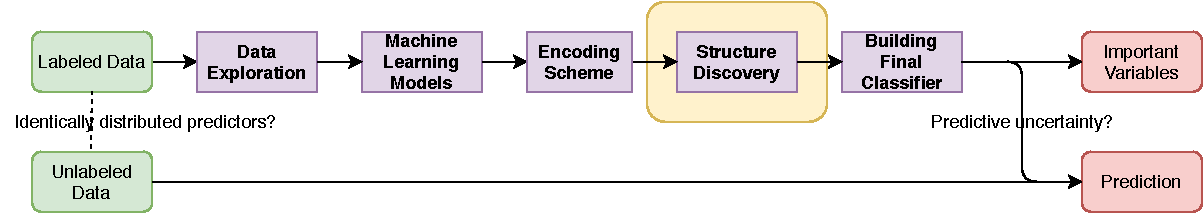
\includegraphics[width=\textwidth]{pipelinenew.pdf}
    \caption{Modeling pipeline.}
    \label{fig:pipeline}
\end{figure}

First, we conduct some routine exploratory data analysis and summarizes the descriptive statistics. Next, we fit popular machine learning models and find linear classifiers outperform the nonparametric models, suggesting a parametric nature of the data. By investigating the coefficients in linear classifiers (linear SVM/logistic regression with $L_1$ penalty), we figure out an ordinal encoding scheme for the categorical variable.

The foregoing analysis alludes some inherent structures of the data. 
On this ground, we develop a novel method called Sparse Grouping Pursuit to automatically discover the sparseness and grouping structure among features. 
This method successfully identifies a single group of important features,
leading to a tremendous dimension reduction. Based on this discovery, we fit a linear SVM which turns out to separate the training data perfectly. Finally, we give the prediction and conduct predictive uncertainty analysis.


\section{Data Analysis}

\subsection{Data Exploration}

\begin{enumerate}

    \item Imbalanced label
    
    The response variable takes a value in classes 0 and 1. 
    Two classes are slightly imbalanced, and about 31\% of training data are in class 1.
    
    \item Distribution of numeric features 
    
    There are 30 numeric features in the data set. 
    All of them have mean zero and standard deviation one, approximately. The Q-Q plots and kernel density estimation plots show that all the numeric features exhibits standard normality, which is further confirmed by the Shapiro-Wilk test. Even for $X_{19}$, the one with the smallest p-value among 30 tests, the empirical density curve is very close to the standard normal distribution, as shown on the left panel of Figure \ref{fig1}.
    
    \item Correlation of numeric features
    
    We calculate the sample Pearson correlation, and find that all features are not correlated. A heatmap of correlation is displayed on the right panel of Figure \ref{fig1}.
    
    \begin{figure}[H]
   \begin{minipage}{0.48\textwidth}
     \centering
     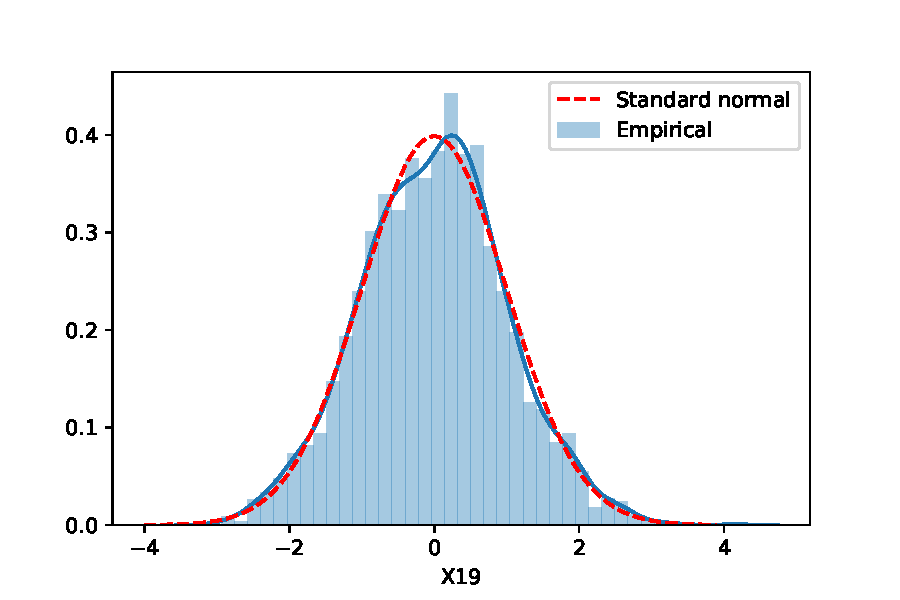
\includegraphics[width=.99\linewidth]{x19.pdf}
   \end{minipage}\hfill
   \begin{minipage}{0.48\textwidth}
     \centering
     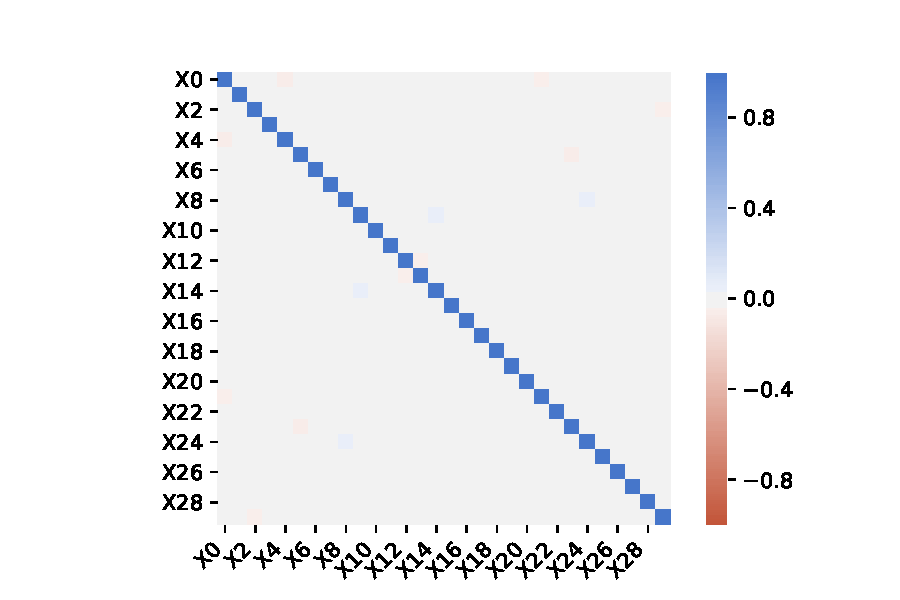
\includegraphics[width=.99\linewidth]{heatmap.pdf}
   \end{minipage}
   \caption{Left: Comparison of empirical density of $X_{19}$ and standard normal. Right: Correlation heatmap.} \label{fig1}
\end{figure}

    
    \item Preliminary variable selection
    
    We compare the boxplots of each numeric feature grouped by class labels. 
    From the visualization, some of features present different quartiles in different classes, indicating a potential influence on the response \cite{li1991sliced}. 
    For example, the plots of $X_4$ and $X_5$ are shown in Figure \ref{fig2}, where $X_4$ is likely to be more influential on the response variable than $X_5$. In this fashion, we identify the following variables that might be of importance: 
    \[X_2,X_3,X_4,X_6,X_7,X_{11},X_{15},X_{17},X_{19},X_{20},X_{21},X_{22},X_{25},X_{26},X_{27}.\]
    
    \begin{figure}[H]
   \begin{minipage}{0.48\textwidth}
     \centering
     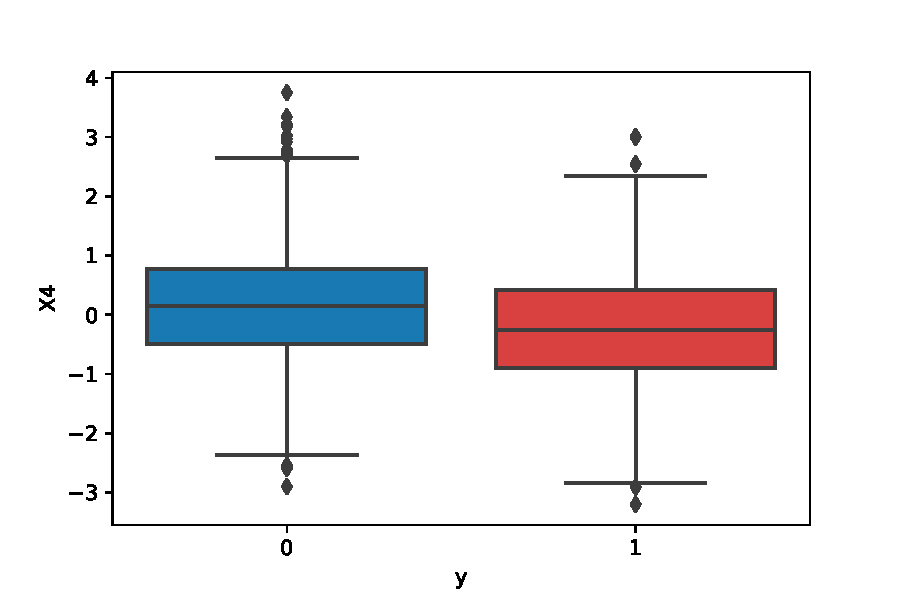
\includegraphics[width=.99\linewidth]{boxplot_x4.pdf}
   \end{minipage}\hfill
   \begin{minipage}{0.48\textwidth}
     \centering
     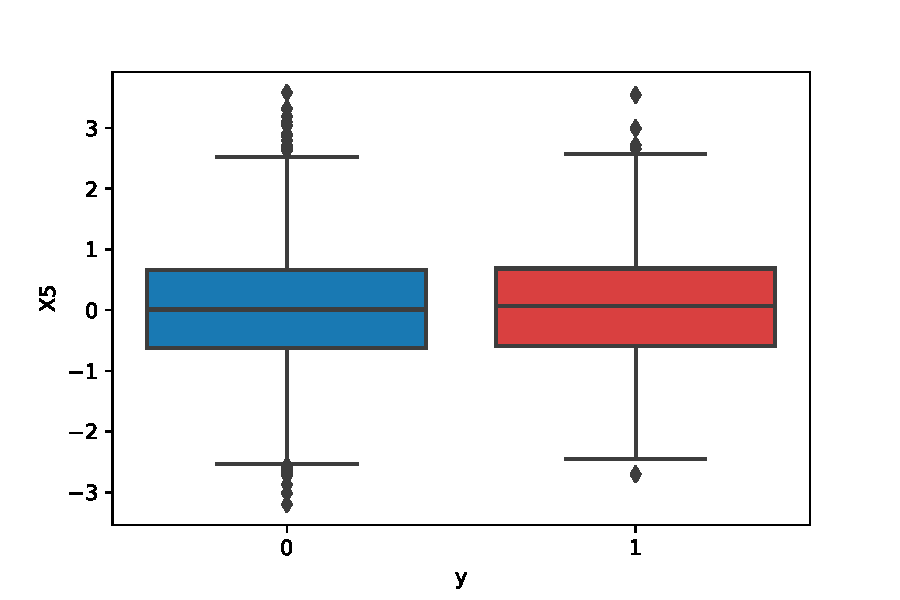
\includegraphics[width=.99\linewidth]{boxplot_x5.pdf}
   \end{minipage}
   \caption{Left: Boxplot of $X_4$. Right: Boxplot of $X_5$.} \label{fig2}
\end{figure}

\item Categorical feature

The data set contains one categorical variable. 
The counts of each factor level are roughly the same, 
suggesting that it may be uniformly sampled from $\{A,B,C,D,E\}$. 
Further, we plot the distribution of the response given each factor level, which shows an ordinal pattern of $\{A,B,C,D,E\}$. More concretely, $X_C=B$ indicates $Y$ is more likely to be $0$ comparing with $X_C=A$. This observation suggests an ordinal numerical encoding scheme may be useful.

\begin{figure}[H]
    \centering
    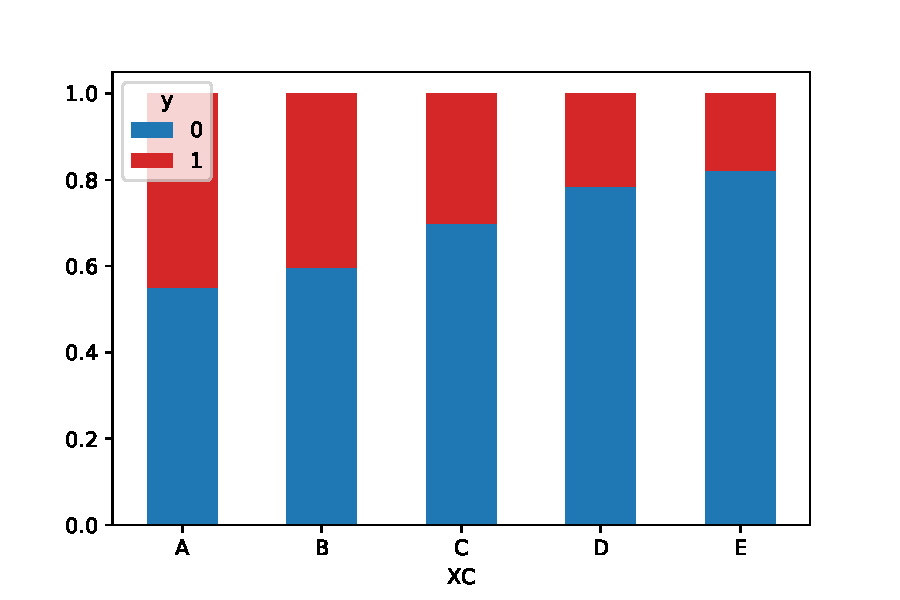
\includegraphics[width=0.7\textwidth]{barplot.pdf}
    \caption{Distribution of $Y$ given $X_C$.}
    \label{fig:barplot}
\end{figure}


\item Identical distribution of the training and testing data

It is important that the training and the testing data are identically distributed in order to make accurate predictions. Therefore, we use the Kolmogorov-Smirnov test to compare the distributions of the training and testing data. It turns out that they are identically distributed. 
\end{enumerate}

The code for exploratory data analysis is in \texttt{eda.ipynb}.


\subsection{Model Fitting and Encoding}

\subsubsection{Coarse Model Comparison}

We commence with multiple candidate models, including Logistic Regression (LR), Linear Discriminant Analysis (LDA), K-Nearest Neighbors (KNN), Classification And Regression Tree (CART), Naive Bayes classifier (NB), Linear Support Vector Machine, LightGBM \cite{ke2017lightgbm}, XGBoost \cite{chen2016xgboost}, and CatBoost \cite{prokhorenkova2018catboost}. Logistic Regression and Linear Support Vector Machine use both $L_1$ and $L_2$ penalty, and the other models use default parameters. To have a comprehensive evaluation of the models, we consider four performance metrics: AUC, Accuracy, F1, and weighted F1. 

As for the encoding of the categorical variable, we start with the most general setting, one-hot encoding, where each factor level is represented by one coefficient. Besides, since the data is imbalanced, although not severe, 10-fold repeated stratified cross validation \cite{scikit-learn} is used. For a fair comparison, the splitting of the folds in cross validation are the same for all models.

The results are shown in Table \ref{tab:model-comparison-onehot}. The models are sorted in a descending order of performances. The linear classifiers, LR, LDA, and SVM, are the best performing models with respect to all four metrics. In contrast, the gradient boosting methods, which are better at modeling nonlinear relationship, perform worse. 
It suggests that the data present a parametric characteristic and
a linear classifier might be more suitable in this situation. 

Figure \ref{fig:onehot_top5} shows the top 5 models and we can see that $L_1$-regularized SVM is the best in terms of every metric, and that $L_1$-regularized Logistic Regression also performs pretty well. Therefore, for the subsequent analysis, we would dig deeper into these two models, in the hope of finding more insights about the data structure. Also note that for both SVM and LR, the $L_1$-regularized versions outperform their $L_2$-regularized counterparts, which reveals the sparsity of features and lays foundation for the further analysis.

\begin{figure}[H]
    \centering
    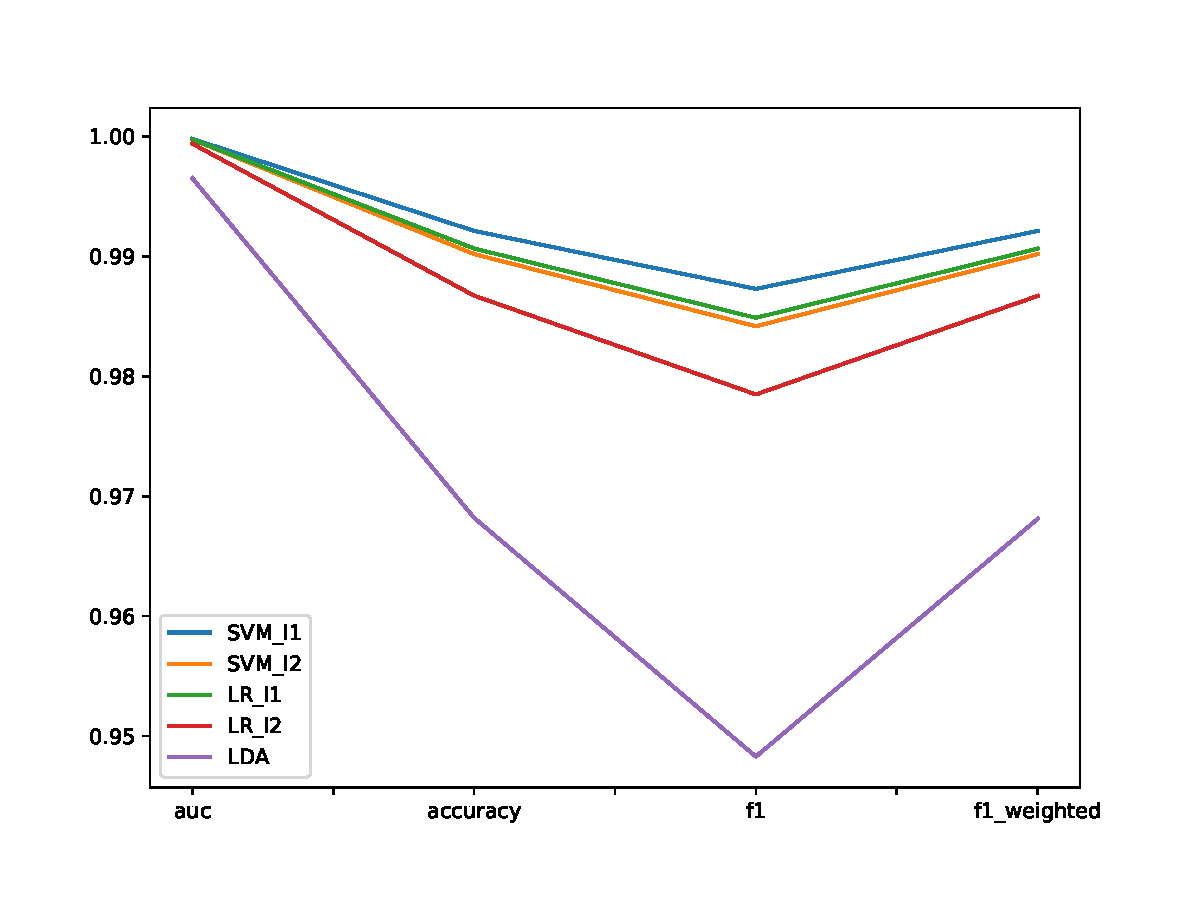
\includegraphics[width=0.7\textwidth]{onehot/top5_model_compare.pdf}
    \caption{Top 5 models using one-hot encoding.}
    \label{fig:onehot_top5}
\end{figure}



\begin{table}[H]
    \centering
    \begin{tabular}{l|c c c c}
        \hline\hline
         & \textsl{AUC} & \textsl{Accuracy} & \textsl{F1} & \textsl{Weighted F1}\\
        \hline
        \textsl{SVM $L_1$} & 0.99981 (0.00020) &  0.99213 (0.00515) &  0.98730 (0.00832) &  0.99213 (0.00516) \\
        \hline
        \textsl{SVM $L_2$} & 0.99976 (0.00024) &  0.99020 (0.00527) &  0.98418 (0.00852) &  0.99020 (0.00527)   \\
        \hline 
        \textsl{LR $L_1$} & 0.99976 (0.00022) &  0.99067 (0.00503) &  0.98488 (0.00818) &  0.99065 (0.00504) \\
        \hline
        \textsl{LR $L_2$} & 0.99941 (0.00045) &  0.98673 (0.00645) &  0.97849 (0.01048) &  0.98671 (0.00646) \\
        \hline
        \textsl{LDA} & 0.99653 (0.00178) & 0.96820 (0.01130) & 0.94828 (0.01839) & 0.96811 (0.01133) \\
        \hline
        \textsl{CatBoost} & 0.98077 (0.00529) & 0.91753 (0.01526) & 0.85211 (0.03036) & 0.91466 (0.01638) \\
        \hline
        \textsl{XGBoost} & 0.96135 (0.00977) & 0.89320 (0.01659) & 0.80863 (0.03263) & 0.88951 (0.01773) \\
        \hline
        \textsl{LGBM} & 0.95764 (0.00979) & 0.88533 (0.01489) & 0.79071 (0.02969) & 0.88057 (0.01596)  \\
        \hline
        \textsl{NB} & 0.93900 (0.01644) & 0.88120 (0.01854) & 0.79454 (0.03449) & 0.87858 (0.01935) \\
        \hline
        \textsl{KNN} & 0.80992 (0.02452) & 0.77253 (0.02054) & 0.54162 (0.05056) & 0.75335 (0.02418) \\
        \hline
        \textsl{CART} & 0.63710 (0.02828) & 0.68807 (0.02409) & 0.49925 (0.04099) & 0.68812 (0.02351) \\
        \hline\hline
    \end{tabular}
    \caption{Model comparison with one-hot encoding (in a descending order).}
    \label{tab:model-comparison-onehot}
\end{table}




\begin{table}[H]
    \centering
    \begin{tabular}{l|c c c c}
        \hline\hline
          & \textsl{AUC} & \textsl{Accuracy} & \textsl{F1} & \textsl{Weighted F1}\\
        \hline
        \textsl{SVM $L_1$} & 0.99986 (0.00015) & 0.99327 (0.00469) & 0.98909 (0.00763) & 0.99326 (0.00470) \\
        \hline
        \textsl{LR $L_1$} & 0.99985 (0.00016) & 0.99233 (0.00412) & 0.98758 (0.00669) & 0.99232 (0.00413)  \\
        \hline
        \textsl{SVM $L_2$} & 0.99980 (0.00019) & 0.99213 (0.00484) & 0.98726 (0.00786) & 0.99212 (0.00485) \\
        \hline
        \textsl{LR $L_2$} & 0.99963 (0.00030) & 0.98967 (0.00496) & 0.98320 (0.00812) & 0.98964 (0.00498) \\
        \hline
        \textsl{LDA} & 0.99692 (0.00169) & 0.97153 (0.01029) & 0.95369 (0.01677) & 0.97145 (0.01032)\\
        \hline
        \textsl{NB} & 0.98924 (0.00436) & 0.90333 (0.01320) & 0.81624 (0.02964) & 0.89773 (0.01497) \\
        \hline
        \textsl{CatBoost} &0.98033 (0.00499) & 0.91860 (0.01452) & 0.85453 (0.02909) & 0.91587 (0.01562) \\
        \hline
        \textsl{XGBoost} & 0.96171 (0.00813) & 0.89047 (0.01543) & 0.80516 (0.02990) & 0.88697 (0.01641)  \\
        \hline
        \textsl{LGBM} & 0.95763 (0.00859) & 0.88560 (0.01454) & 0.79320 (0.03079) & 0.88125 (0.01591) \\
        \hline
        \textsl{KNN} & 0.83402 (0.02241) & 0.79420 (0.01920) & 0.59214 (0.04461) & 0.77845 (0.02195) \\
        \hline
        \textsl{CART} & 0.65175 (0.02424) & 0.70113 (0.02000) & 0.51948 (0.03410) & 0.70117 (0.01972) \\
        \hline\hline
    \end{tabular}
    \caption{Model comparison with ordinal encoding (in a descending order).}
    \label{tab:model-comparison-ordinal}
\end{table}

\subsubsection{Encoding Scheme}
Since $L_1$-regularized SVM model performs the best, and that the estimated coefficients might provide extra information, we decide to dive deeper and check its estimated coefficients. As shown in Table \ref{tab:svm-coef} in Appendix, the coefficients for the one-hot encoded categorical variable are approximately $2.5, 0, -2.5, -5, -7.5$, which suggests that the difference between two adjacent levels are almost the same and hence ordinal encoding might be appropriate. The coefficients plot, as shown in Figure \ref{fig:svm-coef}, further validates our findings.

Therefore, we redo model comparison with the categorical variable encoded by ordinal levels, i.e., $[A, B, C, D, E] \Rightarrow [0, 1, 2, 3, 4]$. Comparing the results in Table \ref{tab:model-comparison-ordinal}, with those using the one-hot encoding scenario (Table \ref{tab:model-comparison-onehot}), we find that almost every model achieves a higher score in terms of every metric, especially for Naive Bayes, which justifies the ordinal encoding. The detailed comparisons among the models using the ordinal encoding scheme are shown in Figures \ref{fig:ordinal_model_compare}-\ref{fig:ordinal_f1_weighted_compare} in Appendix.
In the subsequent analysis, we use the ordinal encoding for $X_C$. 

\begin{figure}[H]
    \centering
    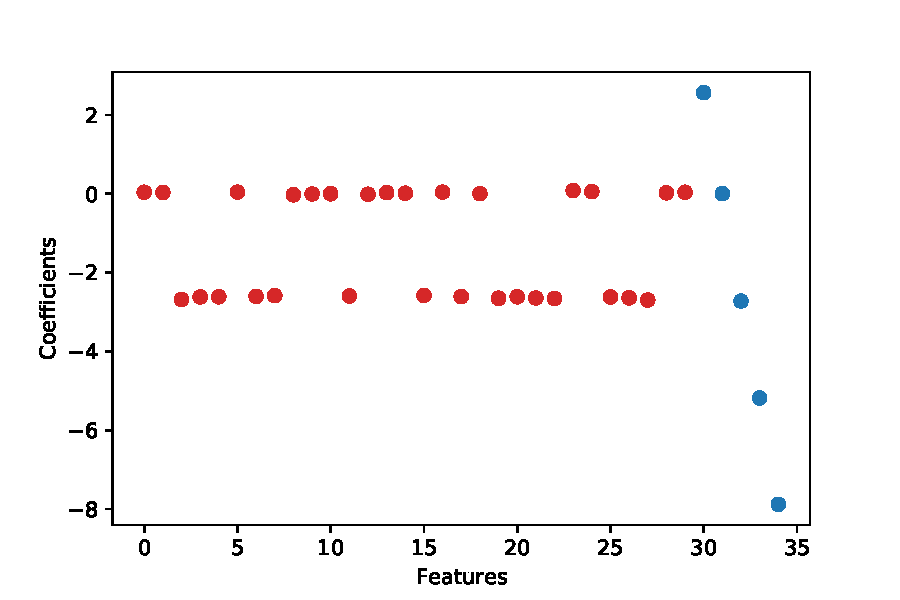
\includegraphics[width=0.7\textwidth]{svm_coef.pdf}
    \caption{Coefficient plot for SVM using one-hot encoding. The coefficients for the categorical feature is in blue.}
    \label{fig:svm-coef}
\end{figure}




\subsection{Structure Discovery: Sparse Grouping Pursuit}

\begin{figure}[H]
    \centering
    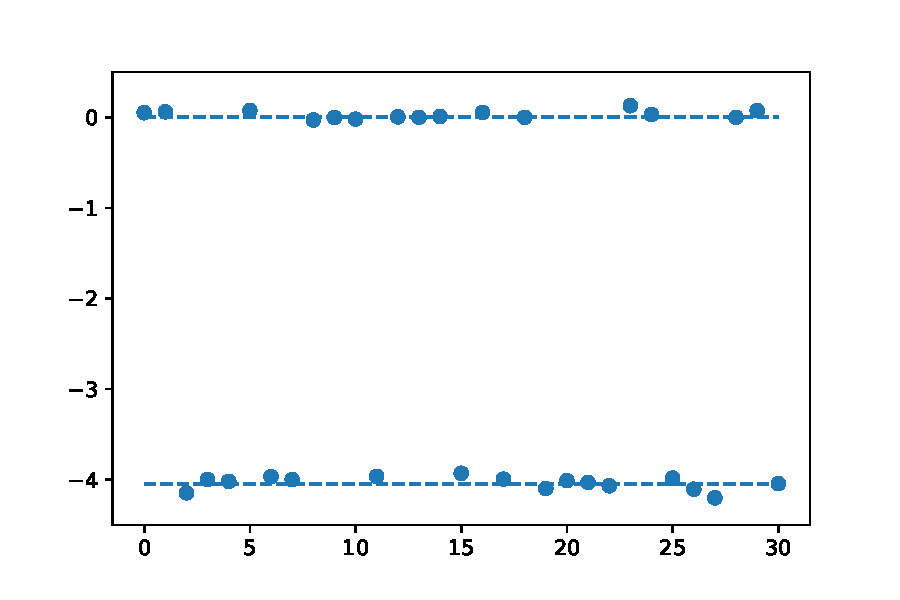
\includegraphics[width=.49\textwidth]{ungroup_coef.pdf}
    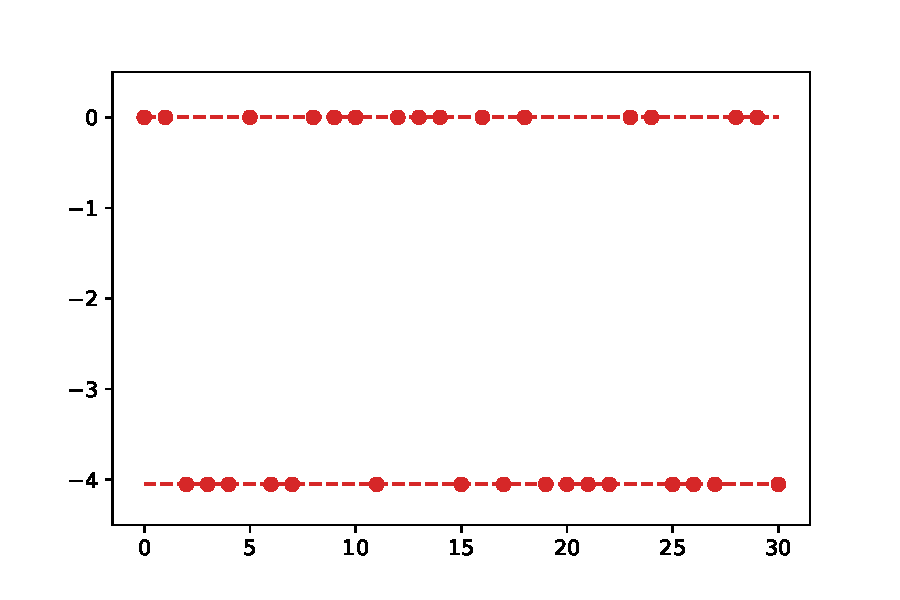
\includegraphics[width=.49\textwidth]{group_coef.pdf}
    \caption{The feature coefficients $\beta$ estimated by the $L_1$ logistic regression (Left) and sparse grouping pursuit logistic regression (Right).}
    \label{fig:coefs}
\end{figure}

To explore the structures of the data, we plot the coefficients estimated by $L_1$ regularized logistic regression. As shown in Figure \ref{fig:coefs} (Left), the estimated coefficients are divided into two clusters: one cluster is centered around $0$, while the other is centered around $-4$. 
It suggests that some features might share the same coefficients. 

On this ground, we generalize the Grouping Pursuit \cite{shen2010grouping},
referred to as Sparse Grouping Pursuit.
Specifically, the estimator is given by
\begin{equation}\label{model:sparse-group-pursuit}
    (\widehat\beta_0, \widehat\beta) = \arg\min_{\beta_0,\beta} \ \textnormal{Loss}(\beta_0,\beta)
    + \lambda(\textnormal{Pen}_0(\beta) + \textnormal{Pen}_G(\beta)),
\end{equation}
where $\beta_0\in\mathbf{R}$ is an intercept, $\beta = (\beta_1,\ldots,\beta_d)\in\mathbf{R}^d$ are coefficients of features, and
\begin{equation}\label{model:penalty}
    \textnormal{Pen}_0(\beta) = \sum_{j=1}^d \min(|\beta_j|/\tau,1),
    \quad
    \textnormal{Pen}_G(\beta) = \sum_{j<j'} \min(|\beta_j - \beta_{j'}|/\tau,1).
\end{equation}
In \eqref{model:penalty}, the loss function can be any large margin loss (e.g. logistic loss), and $\lambda>0$ and $\tau>0$ are tuning parameters, which can be selected by cross-validation. 

Importantly, $\text{Pen}_0$ penalizes on the magnitude of $\beta_j$ when $|\beta_j|$ is smaller than a threshold $\tau$, 
but leaves the penalty of $\beta_j$ constant when $|\beta_j|$ is larger than $\tau$. This will induce sparsity but avoid over-penalization on the estimate. 
Similarly, $\text{Pen}_G$ penalizes on the differences $|\beta_j-\beta_{j'}|$ when it is smaller than $\tau$, 
but does not impose any more penalty when it is larger than $\tau$.
This helps in detecting the potential groups, 
but avoid false grouping caused by over-penalization where all coefficients are pushed together. 


The Sparse Grouping Pursuit is a general method for sparse and group structured data. Figure \ref{fig:coefs} (Right) shows that the features are divided into two index groups by Sparse Grouping Pursuit, 
\begin{equation*}
    \begin{split}
        G_0 &= \{ 0,1,5,8,9,10,12,13,14,16,18,23,24,28,29 \},\\
        G_1 &= \{ 2,3,4,6,7,11,15,17,19,20,21,22,25,26,27,30 \}.
    \end{split}
\end{equation*}
where the features in a group have the same coefficients. 
In particular, $G_0$ includes all features with zero coefficient.
Therefore, Sparse Grouping Pursuit automatically detects the sparsity and the group structure in the data.



{\bf Remark.}
The statistical properties of Sparse Grouping Pursuit are inherited from the original Grouping Pursuit \cite{shen2010grouping}. 
For computation, \eqref{model:sparse-group-pursuit} can be effectively solved by
combining the Majorization Minimization algorithm \cite{hunter2000quantile} using the Local Linear Approximation \cite{zou2008one} (MM-LLA) and
the Alternating Direction Method of Multipliers (ADMM) \cite{boyd2011distributed}.
The program code for solving \eqref{model:sparse-group-pursuit} is included in \texttt{group.py}. 


\subsection{Final Classifier: Separating Hyperplane}

Suppose $G_0,\ldots, G_L$ are groups discovered by the Sparse Grouping Pursuit, 
where $G_{k}\cap G_{k'}=\emptyset$ and $\bigcup_{k=0}^{L}G_k = \{1,\ldots,d\}$. 
Let $G_0$ be the group of features with zero coefficients. 
Then the discovered group structure helps to reduce the dimension of the model further. In particular, we define the grouped features 
$Z_{k} = \sum_{j\in G_k} X_j$; $k=1,\ldots,L$.
Then we fit a prediction model (e.g. SVM) based on $Z=(Z_1,\ldots,Z_L)$. 


Since the Sparse Grouping Pursuit discovered groups $G_0$ and $G_1$, 
we define a new feature $Z_1$ and plot the response $Y$ against $Z_1$ in Figure \ref{fig:Bayes}. Remarkably, the data are linearly separable. 
Therefore, we consider constructing a separating hyperplane that maximizes the margin of two classes (i.e., linearly separable SVM):
\begin{equation}\label{model:bayes}
    \widehat C(Z_1) = 0.5\times (1 - \textnormal{Sign}(Z_1)).
\end{equation}
Then model \eqref{model:bayes} is used for final prediction and the prediction result is in \texttt{pred.csv}.

\subsection{Predictive Uncertainty}

It is exciting that our model fits the data perfectly on the training set. Meanwhile, we would like to quantify the confidence of our model on the test set. Since the final classifier \eqref{model:bayes} is a one-dimensional SVM, we inspect its margin to assess the prediction uncertainty. Generally, a larger margin implies a more robust classifier. For points outside the margin, we would be more confident in the prediction, while for points inside the margin, they are more likely to be misclassified.

For the training data, we obtain a margin $[-2.75\times 10^{-3}, 1.33 \times 10^{-3}]$. Applying model \eqref{model:bayes} to the test set, we find that only one point (out of 7000) falls inside this margin, with $Z_1 = -3.58 \times 10^{-4}$. 
Based on this, we estimate the predicted F1 score would be in $[0.9997, 1.0]$.

\begin{figure}[H]
    \centering
    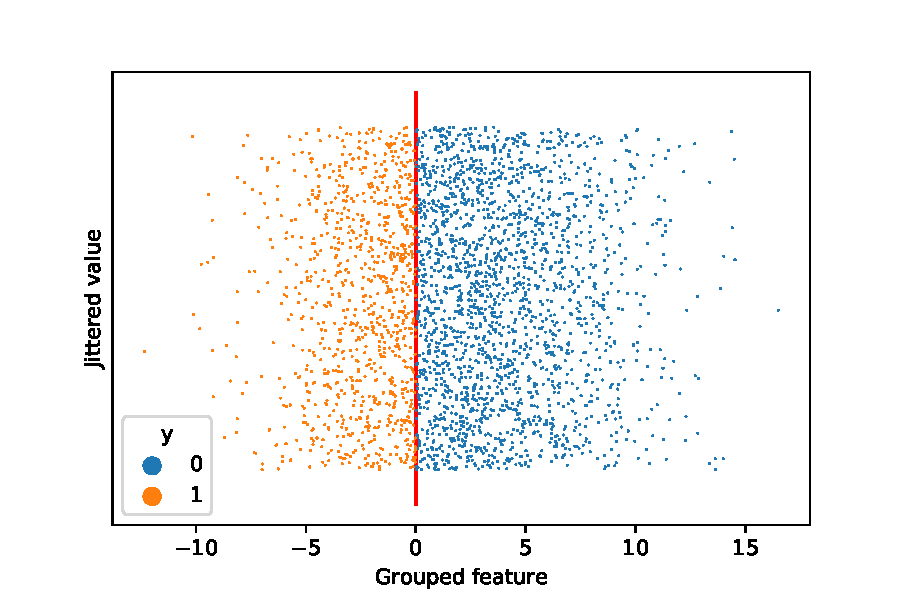
\includegraphics[width=.49\linewidth]{Bayesorigin.pdf}
    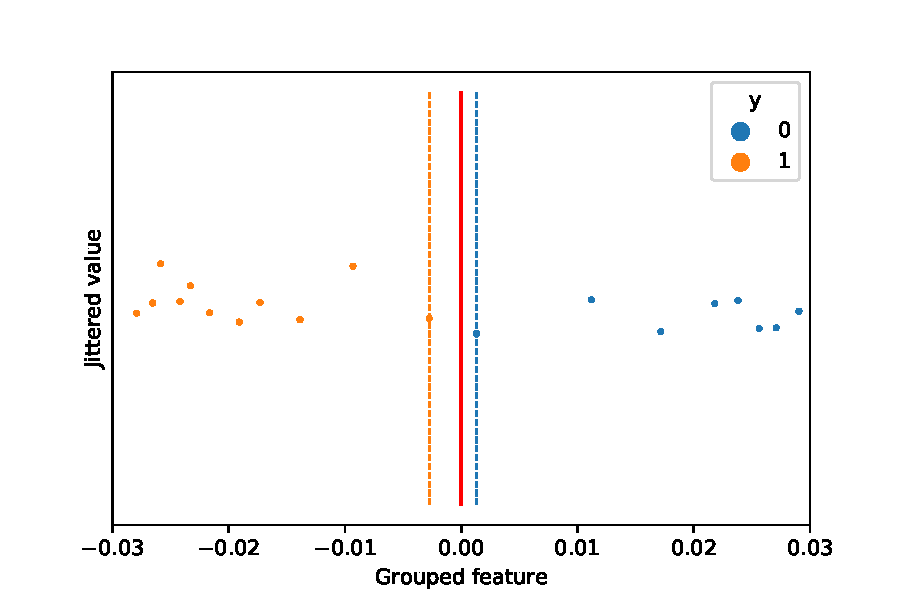
\includegraphics[width=.49\linewidth]{Bayeszoomin.pdf}
   \caption{Left: Training set is linearly separable (The vertical axis has no actual meaning.) Right: Zoomed in of the left panel}    \label{fig:Bayes}
\end{figure}

\section{Conclusion and Discussion}

\subsection{Conclusion}

In this challenge, we start with data exploration to examine  data distribution and identify the data patterns. Then by model comparison, we find that $L_1$-regularized SVM and Logistic Regression outperform the other models, and that ordinal encoding scheme yields better performance than one-hot encoding. With the insights obtained in the preceding analysis, we develop a novel method, Sparse Grouping Pursuit, to investigate the inherent parametric structures. The features
\begin{equation*}
    X_2,X_3,X_4,X_6,X_7,X_{11},X_{15},X_{17},X_{19},X_{20},X_{21},X_{22},X_{25},X_{26},X_{27},X_C
\end{equation*}
form a least set of informative feature variables as well as a single group, reducing the dimension of the feature space to one and leading to a linearly separable case. Applying the final classifier to the training set, we get a perfect F1 score being 1. The predictive uncertainty analysis shows a high confidence of the prediction on the test set.

\subsection{Strengths and Limitations}
With a perfect F1 score on the training set, one may raise concerns of overfitting, but this will not be the case. 
Our method focuses on digging out the inherent structure of the data and the resulting final model is actually a linear classifier with dimension one, having low variance statistically (in terms of bias-variance tradeoff). We would credit our success to the Sparse Grouping Pursuit.

 In this challenge, the Sparse Grouping Pursuit is developed for a specific classification task, but it is versatile. It can be easily generalized to other cases where the response is continuous, binomial, multinomial, poisson and so on. As long as a parametric base model is valid, it can be used to find out the inner structure of the data. Meanwhile, the limitation is apparent in that it is not applicable for non-parametric models. We would suggest consider model averaging to combine the insights from both parametric and non-parametric models if non-parametric models turn out to have dominant performances.
 
\subsection{Potential Applications}
There are two main usages of the Sparse Grouping Pursuit, reducing dimension and handling multicollinearity. 
In terms of the former, with the help of Sparse Grouping Pursuit, 
one can effectively reduce the dimension to the number of groups, and detect low dimensional sparse signals. For example, in gene network analysis where the data is usually high-dimensional, our method can identify homogeneous subnetworks, which would substantially deduct dimension of features and hence help with understanding a disease.

For multicollinearity, if not handled appropriately, it will increase the uncertainty in both estimation and prediction, rendering unreliable and nonrobust results. Specifically, many models in finance, e.g. credit card fraud detection models, are built on top of a wide source of information and it is very likely that these features are highly correlated.
With fine-tuned hyper-parameters, Sparse Grouping Pursuit is able to group and aggregate the highly linearly correlated variables. In this way, the multicollinearity issue will be greatly alleviated.
Thus, our method can help to stabilize the estimation and prediction of the models and yield more robust results.
    
\subsection{Miscellaneous}
Gradient Boosting methods are not necessarily the top one choice when building a model. Sometimes, simple linear models may have better performance if the data nature is linear, such as this project. The key to build good models should always lie in discovering and exploiting the inherent characteristics of the data.


\bibliography{ref}

\newpage
\appendix

\section{Tables}

\begin{table}[H]
    \centering
    \begin{tabular}{|c|c|c|c|c|c|c|}
         \hline
         $X_0$	& $X_1$	& $X_2$	& $X_3$	& $X_4$	& $X_5$	& $X_6$	\\
         \hline
         0.036534 & 0.030191 & -2.680076 & -2.617866 & -2.614526 & 0.040446 & -2.603064 \\
         \hline
         $X_7$	& $X_8$	& $X_9$	& $X_{10}$	& $X_{11}$	& $X_{12}$	& $X_{13}$	\\
         \hline
         -2.585802 & -0.027194 & -0.00686 & 0.0 & -2.595467 & -0.014203 & 0.026846 \\
         \hline
         $X_{14}$	& $X_{15}$	& $X_{16}$	& $X_{17}$	& $X_{18}$	& $X_{19}$	& $X_{20}$	\\
         \hline
         0.012906 & -2.579457 & 0.04015 & -2.608736 & 0.000415 & -2.652319 & -2.613898 \\
         \hline
         $X_{21}$	& $X_{22}$	& $X_{23}$	& $X_{24}$	& $X_{25}$	& $X_{26}$	& $X_{27}$	\\
         \hline
         -2.645435 & -2.65635 & 0.080488 & 0.053938 & -2.619766 & -2.641279 & -2.697076 \\
         \hline
         $X_{28}$	& $X_{29}$	& A	& B	& C	& D	& E	\\
         \hline
         0.022468 & 0.036541 & 2.565274 & 0.001774 & -2.722318 & -5.181473 & -7.881363 \\
         \hline
    \end{tabular}
    \caption{Estimated coefficients by $L_1$-regularized linear SVM.}
    \label{tab:svm-coef}
\end{table}





\section{Figures}

\begin{figure}[H]
    \centering
    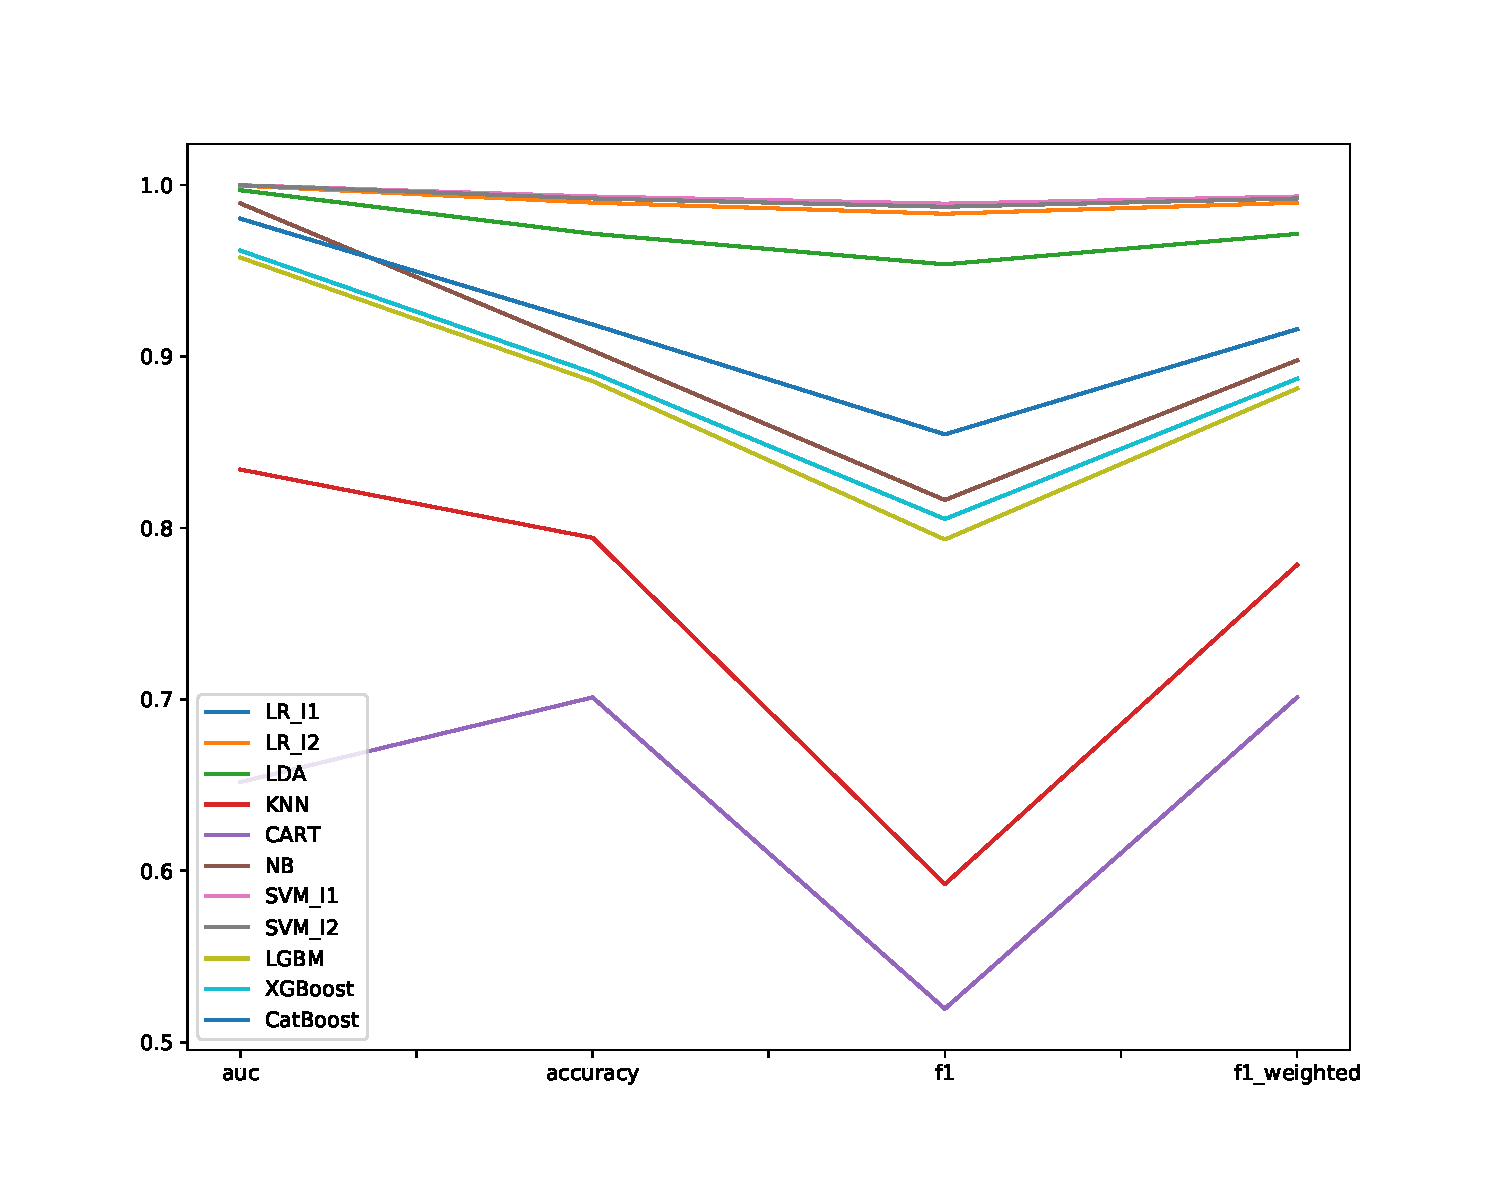
\includegraphics[width=0.75\textwidth]{ordinal/model_compare.pdf}
    \caption{Model comparison using ordinal encoding.}
    \label{fig:ordinal_model_compare}
\end{figure}


\begin{figure}[H]
    \centering
    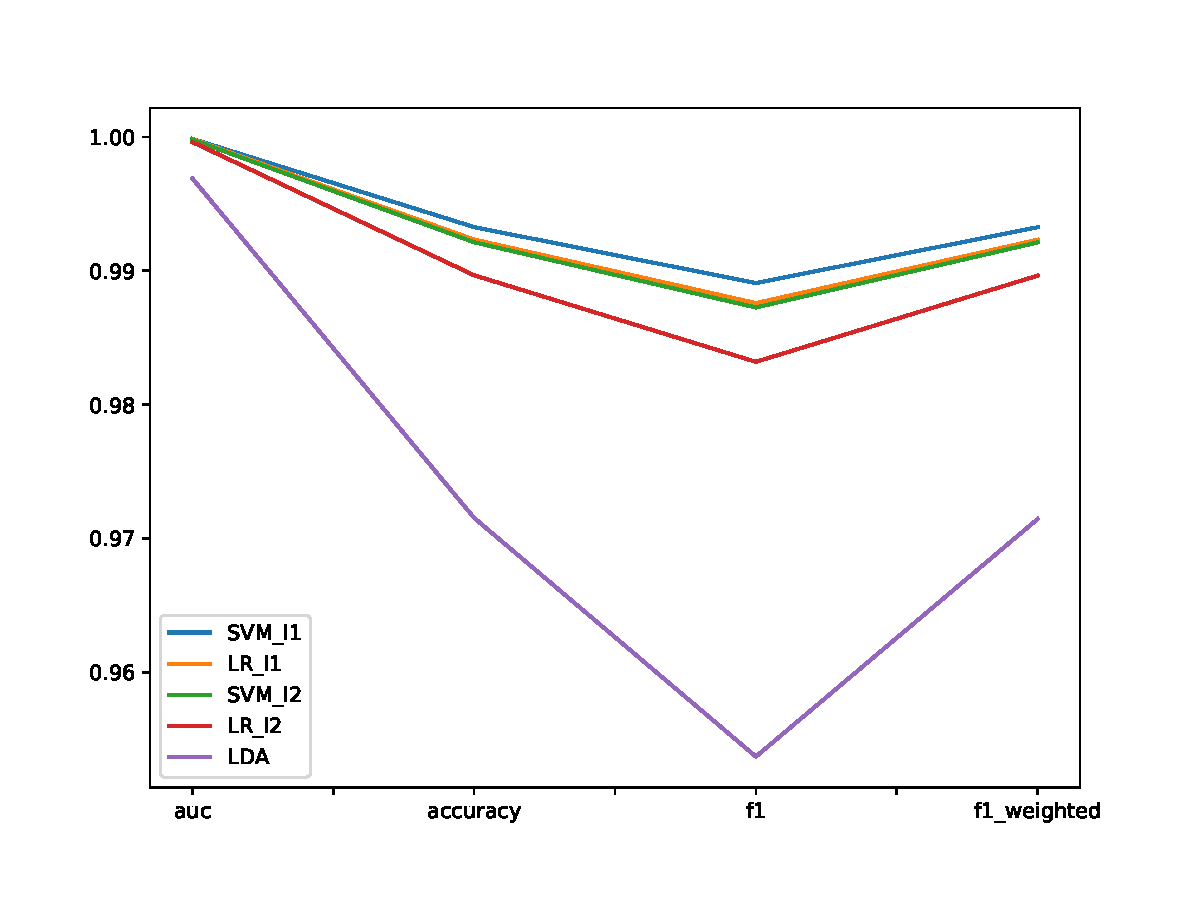
\includegraphics[width=0.75\textwidth]{ordinal/top5_model_compare.pdf}
    \caption{Top 5 models using ordinal encoding.}
    \label{fig:ordinal_top5_compare}
\end{figure}


\begin{figure}[H]
    \centering
    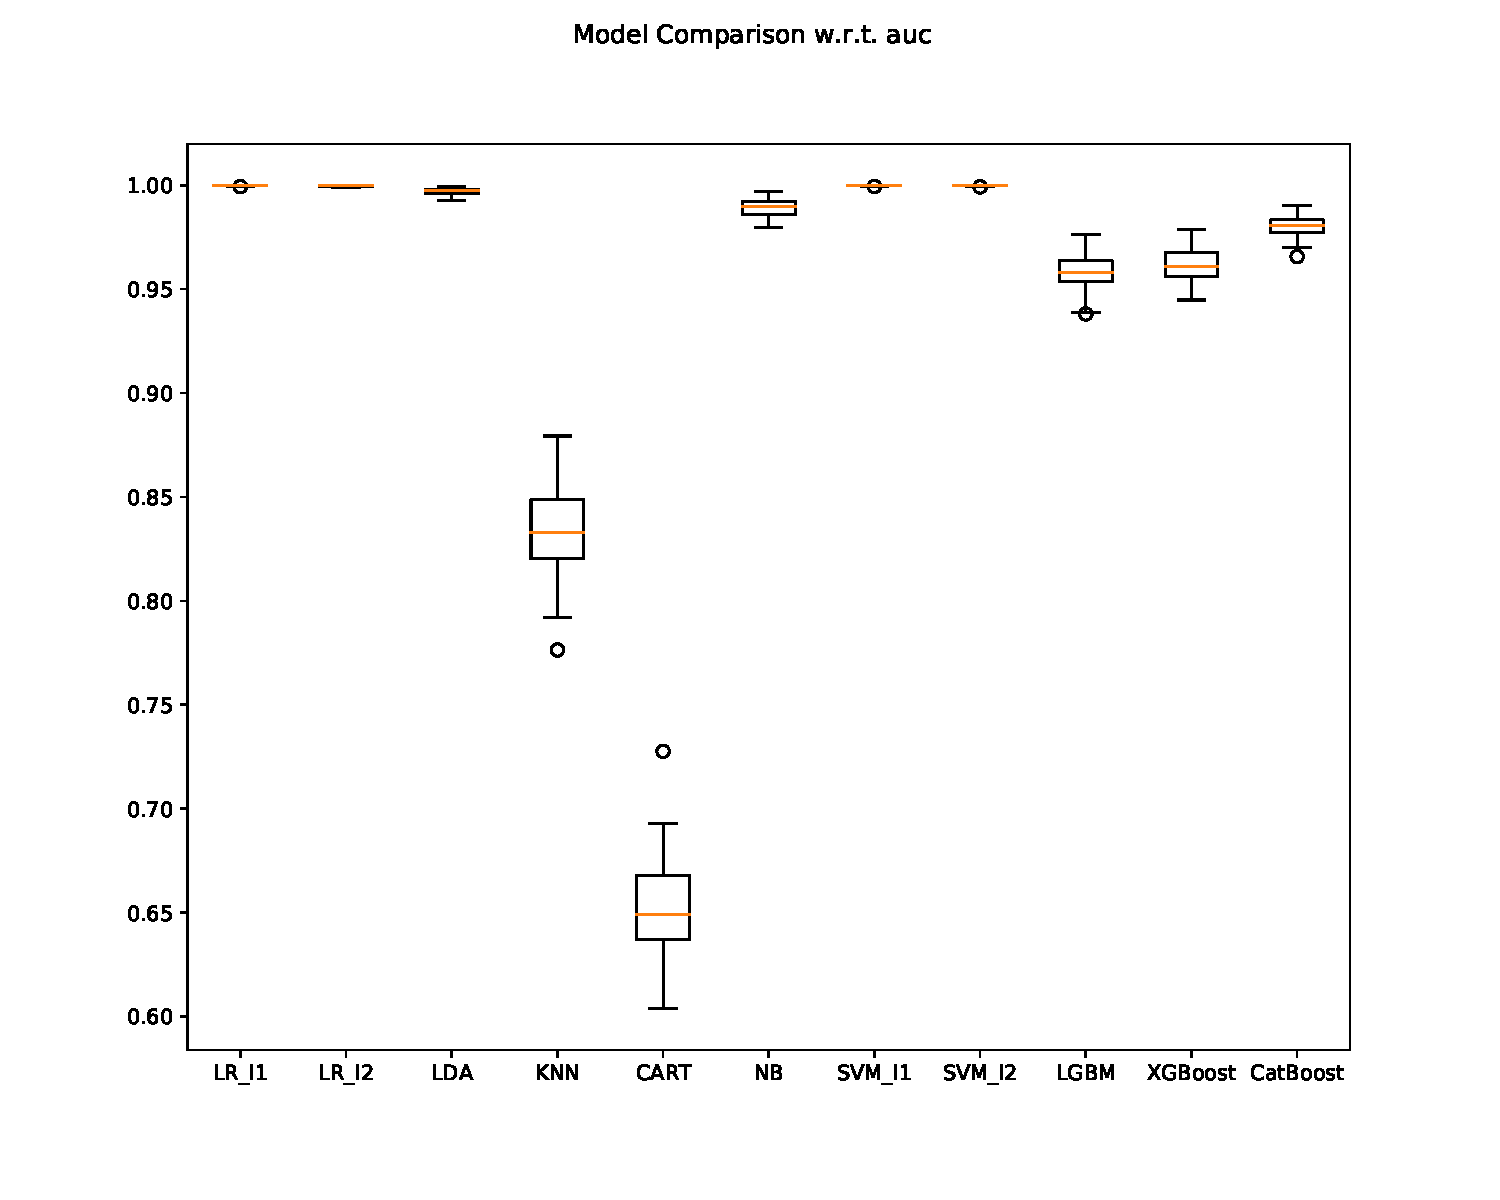
\includegraphics[width=0.75\textwidth]{ordinal/model_compare_auc.pdf}
    \caption{Model comparison in AUC using ordinal encoding.}
    \label{fig:ordinal_auc_compare}
\end{figure}

\begin{figure}[H]
    \centering
    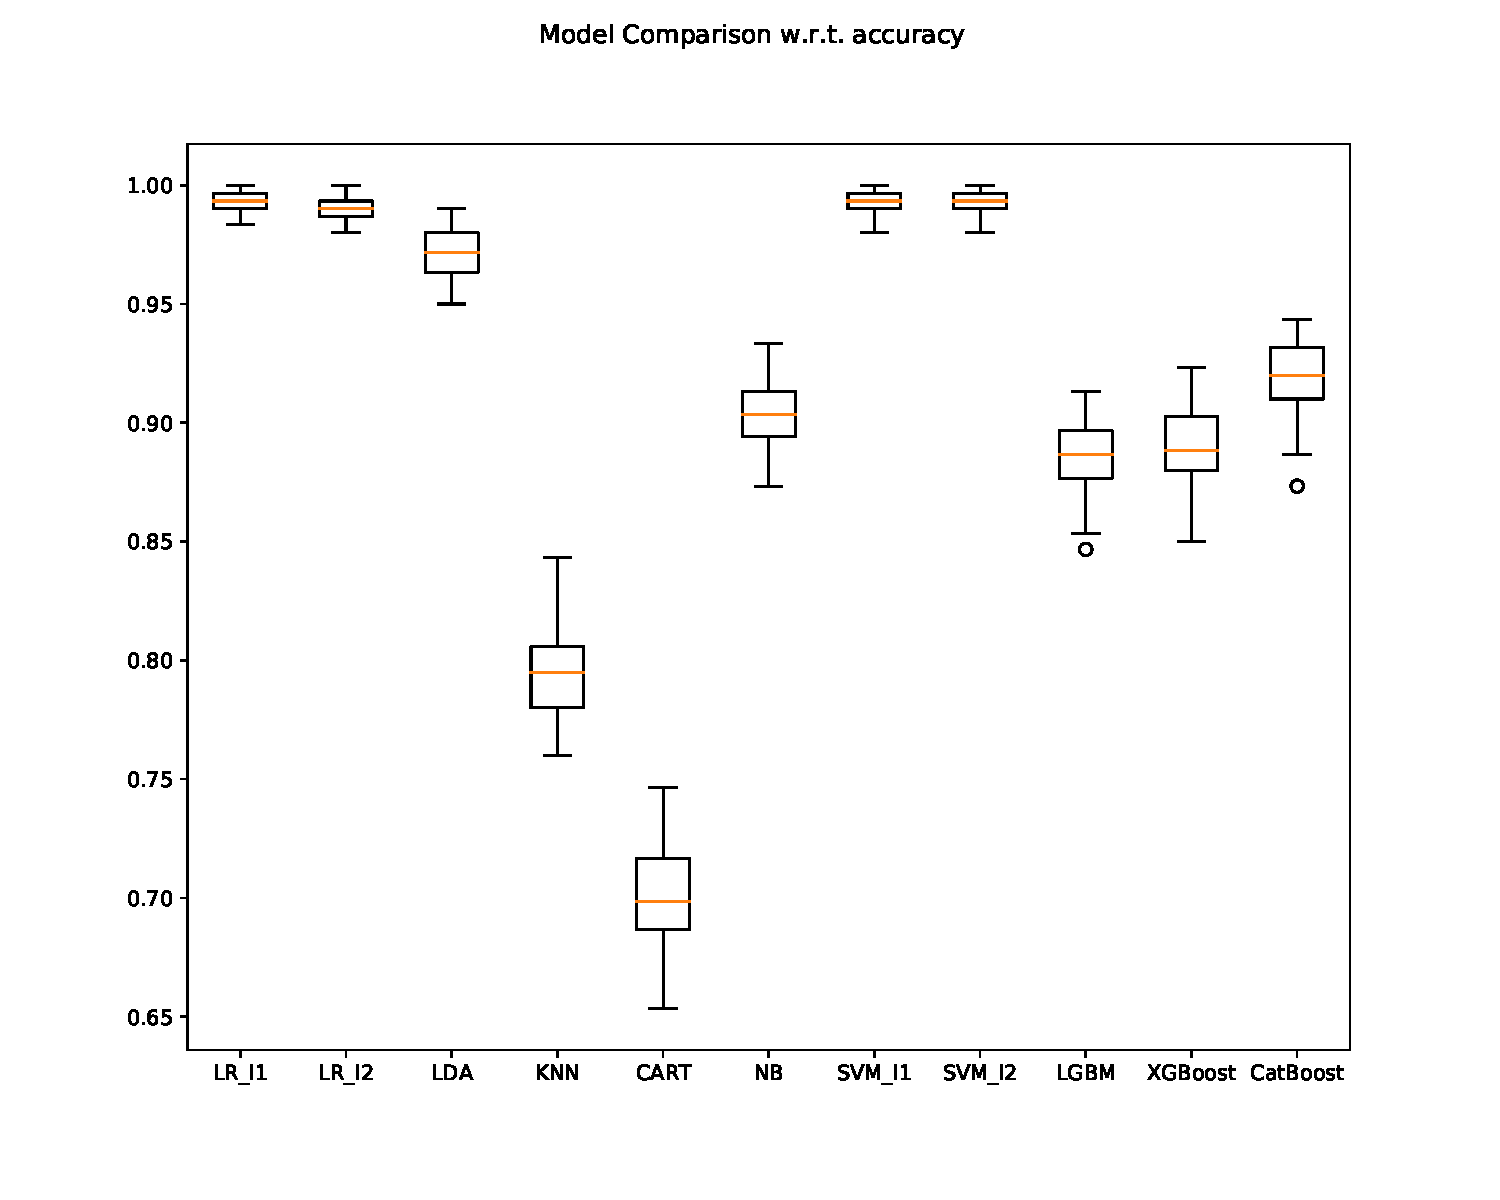
\includegraphics[width=0.75\textwidth]{ordinal/model_compare_accuracy.pdf}
    \caption{Model comparison in Accuracy using ordinal encoding.}
    \label{fig:ordinal_accuracy_compare}
\end{figure}

\begin{figure}[H]
    \centering
    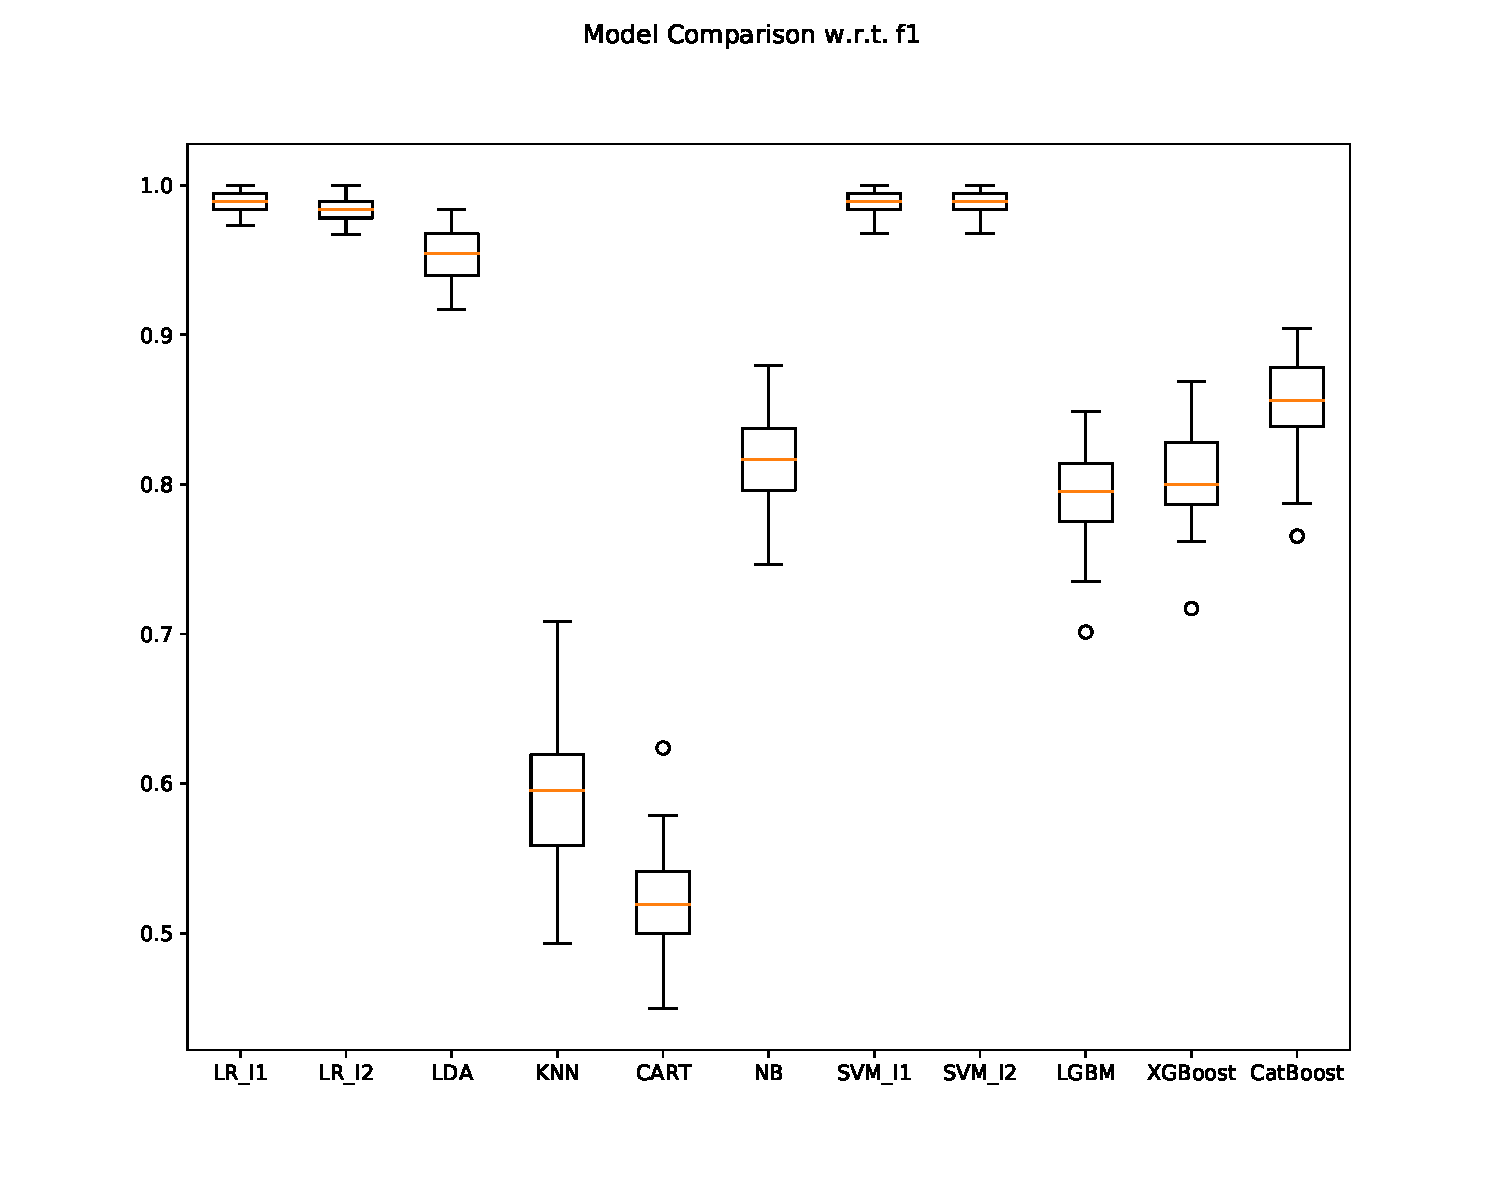
\includegraphics[width=0.75\textwidth]{ordinal/model_compare_f1.pdf}
    \caption{Model comparison in F1 using ordinal encoding.}
    \label{fig:ordinal_f1_compare}
\end{figure}

\begin{figure}[H]
    \centering
    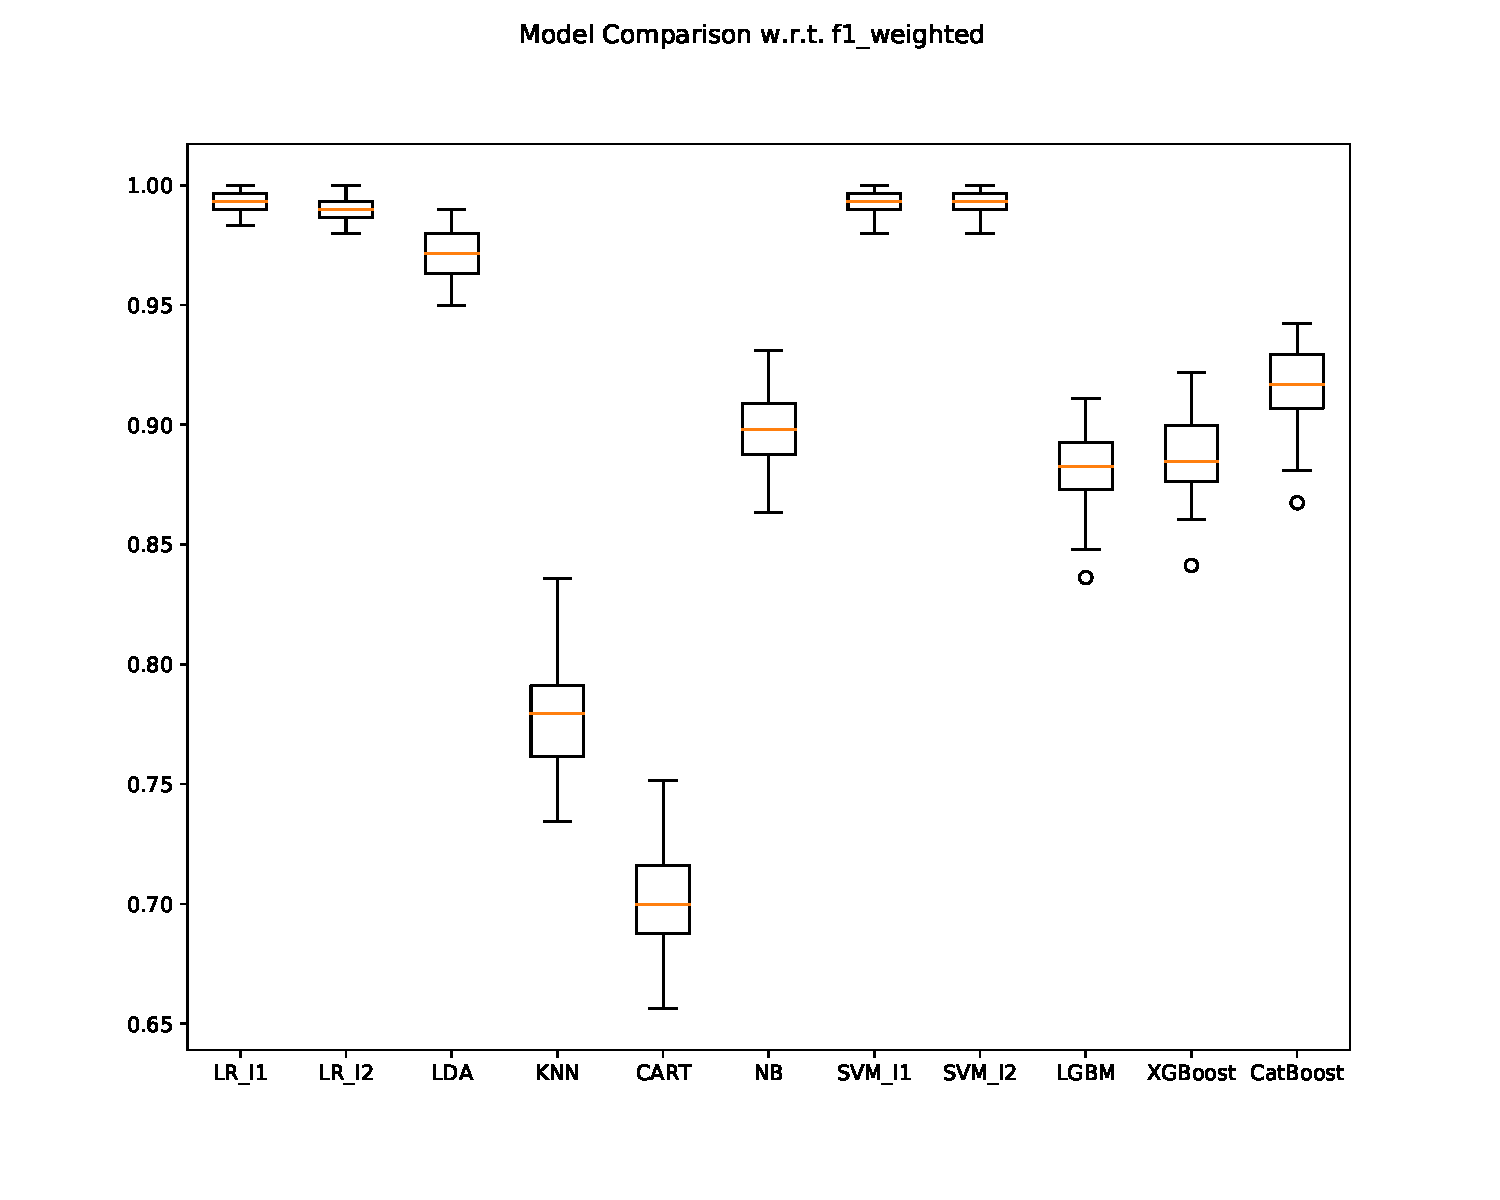
\includegraphics[width=0.75\textwidth]{ordinal/model_compare_f1_weighted.pdf}
    \caption{Model comparison in F1-weighted using ordinal encoding.}
    \label{fig:ordinal_f1_weighted_compare}
\end{figure}


\section{Code}

\begin{enumerate}
    \item The final prediction file is \texttt{pred.csv}.
    \item Exploratory data analysis is implemented in \texttt{eda.ipynb}.
    \item The code for fitting Sparse Grouping Pursuit is in \texttt{group.ipynb}.
    \item The code for modeling, encoding, and predicting is in \texttt{models.ipynb}.
    \item The functions utilized are in \texttt{group.py} and \texttt{models.py}.
    \item The conda environment configuration file is \texttt{environment.yml}.
\end{enumerate}

\end{document}